\chapter{\IfLanguageName{dutch}{Stand van zaken}{State of the art}}%
\label{ch:stand-van-zaken}
\section{Databeschrijving vooraf}{\label{sec:dataopstelling}}
Om aan de slag te gaan met deze bachelorproef is het belangrijk om te weten welke data er gebruikt wordt en hoe deze data is opgebouwd.
In het begin van de bachelorproef was de gekregen data een SAP-boomstructuur die alle onderdelen van het productieproces bevatte.
Deze JSON-file met data was enorm groot (+50.000 JSON-objecten) en uitgebreid (veel eigenschappen per object), wat het developmentproces voor het maken van de chatbot zelf bemoeilijkte.
Daarom is er gebruik gemaakt van een mock-data subset die dezelfde structuur vormt als de originele data, maar met fictieve sleutel-waarde paren.

Voor de opbouw van het project maakt dit verder geen verschil, de scripts in Javascript en Python zijn generiek geschreven waardoor elke data met dezelfde structuur kan worden gebruikt.
Deze structuur begint meestal vanuit een JSON-bestand die omgezet wordt via een Python script naar JSON-LD formaat.
In figuur~\ref{fig:graphmodel} is een voorbeeld te zien van de mock-data in grafiekvorm die is gebruikt in deze bachelorproef.

% Tip: Begin elk hoofdstuk met een paragraaf inleiding die beschrijft hoe
% dit hoofdstuk past binnen het geheel van de bachelorproef. Geef in het
% bijzonder aan wat de link is met het vorige en volgende hoofdstuk.

% Pas na deze inleidende paragraaf komt de eerste sectiehoofding.

% Dit hoofdstuk bevat je literatuurstudie. De inhoud gaat verder op de inleiding, maar zal het onderwerp van de bachelorproef *diepgaand* uitspitten. De bedoeling is dat de lezer na lezing van dit hoofdstuk helemaal op de hoogte is van de huidige stand van zaken (state-of-the-art) in het onderzoeksdomein. Iemand die niet vertrouwd is met het onderwerp, weet nu voldoende om de rest van het verhaal te kunnen volgen, zonder dat die er nog andere informatie moet over opzoeken \autocite{Pollefliet2011}.

% Je verwijst bij elke bewering die je doet, vakterm die je introduceert, enz.\ naar je bronnen. In \LaTeX{} kan dat met het commando \texttt{$\backslash${textcite\{\}}} of \texttt{$\backslash${autocite\{\}}}. Als argument van het commando geef je de ``sleutel'' van een ``record'' in een bibliografische databank in het Bib\LaTeX{}-formaat (een tekstbestand). Als je expliciet naar de auteur verwijst in de zin (narratieve referentie), gebruik je \texttt{$\backslash${}textcite\{\}}. Soms is de auteursnaam niet expliciet een onderdeel van de zin, dan gebruik je \texttt{$\backslash${}autocite\{\}} (referentie tussen haakjes). Dit gebruik je bv.~bij een citaat, of om in het bijschrift van een overgenomen afbeelding, broncode, tabel, enz. te verwijzen naar de bron. In de volgende paragraaf een voorbeeld van elk.

% \textcite{Knuth1998} schreef een van de standaardwerken over sorteer- en zoekalgoritmen. Experten zijn het erover eens dat cloud computing een interessante opportuniteit vormen, zowel voor gebruikers als voor dienstverleners op vlak van informatietechnologie~\autocite{Creeger2009}.

% Let er ook op: het \texttt{cite}-commando voor de punt, dus binnen de zin. Je verwijst meteen naar een bron in de eerste zin die erop gebaseerd is, dus niet pas op het einde van een paragraaf.
\section{Technische specificaties}
In dit eerste hoofdstuk worden de technische specificaties van de verschillende technologieën die gebruikt in deze bachelorproef besproken.
Hierbij wordt dieper ingegaan op het gebruik van CosmosDB, NodeJS, Gremlin API en de verschillende modellen die gebruikt worden om de data te structureren en te analyseren.
Ook worden andere technische mogelijkheden die getest zijn (maar niet gebruikt met bepaalde redenen) besproken.

\subsection{Grafiekmodellering}
Grafiekmodellering is een techniek die gebruikt wordt om de data te visualiseren en te analyseren. Deze data wordt opgeslagen in een grafiekdatabase zoals CosmosDB~\autocite{neo4j20252}. 
In deze bachelorproef wordt dit gebruikt om de verbanden te leggen tussen de verschillende processen binnen ArcelorMittal Gent.
Dit gebeurt door middel van één of meerdere knopen die verbonden zijn met andere knopen doormiddel van een relatie.
Een knoop stelt een entiteit voor, zoals een persoon, een product of een proces. Een verbinding stelt de relatie tussen de verschillende knopen voor zoals een associatie, transformatie of transactie van een product~\autocite{Byun2020}.
Dit kan in ons geval een kraan zijn die verbonden is met een machine. Hierbij zijn de kraan en de machine de knopen en is de relatie een associatie tussen deze knopen.
Om de traceerbaarheid te behouden wordt bij het wijzigen van een knoop ook de tijdstempel opgeslagen van deze wijziging, zodat er altijd kan worden opgevraagd wanneer deze knoop is gewijzigd.
De relatie zal in dit geval worden omgezet naar een ``has-event''-relatie die een ``delete event'' bevat, zegt~\autocite{Byun2020}.

Elke knoop bevat ook eigenschappen die zichzelf beschrijven. Dit kan bijvoorbeeld het bouwjaar, laatste onderhoud of zelfs sensordata, zoals een alarm op de machine.
Deze data wordt opgeslagen als sleutel-waarde paar om dit later efficiënt te kunnen ophalen, door in de query te vragen naar de sleutelwaarde.
in figuur~\ref{fig:graphmodel} is een voorbeeld te zien van een grafiekmodel met fictieve data dat opgezet is in CosmosDB.\@
Daarnaast is er in schema~\ref{fig:workflow} een visuele voorstelling van de workflow van de chatbot die is opgezet.

\begin{figure}[H]
     \centering
     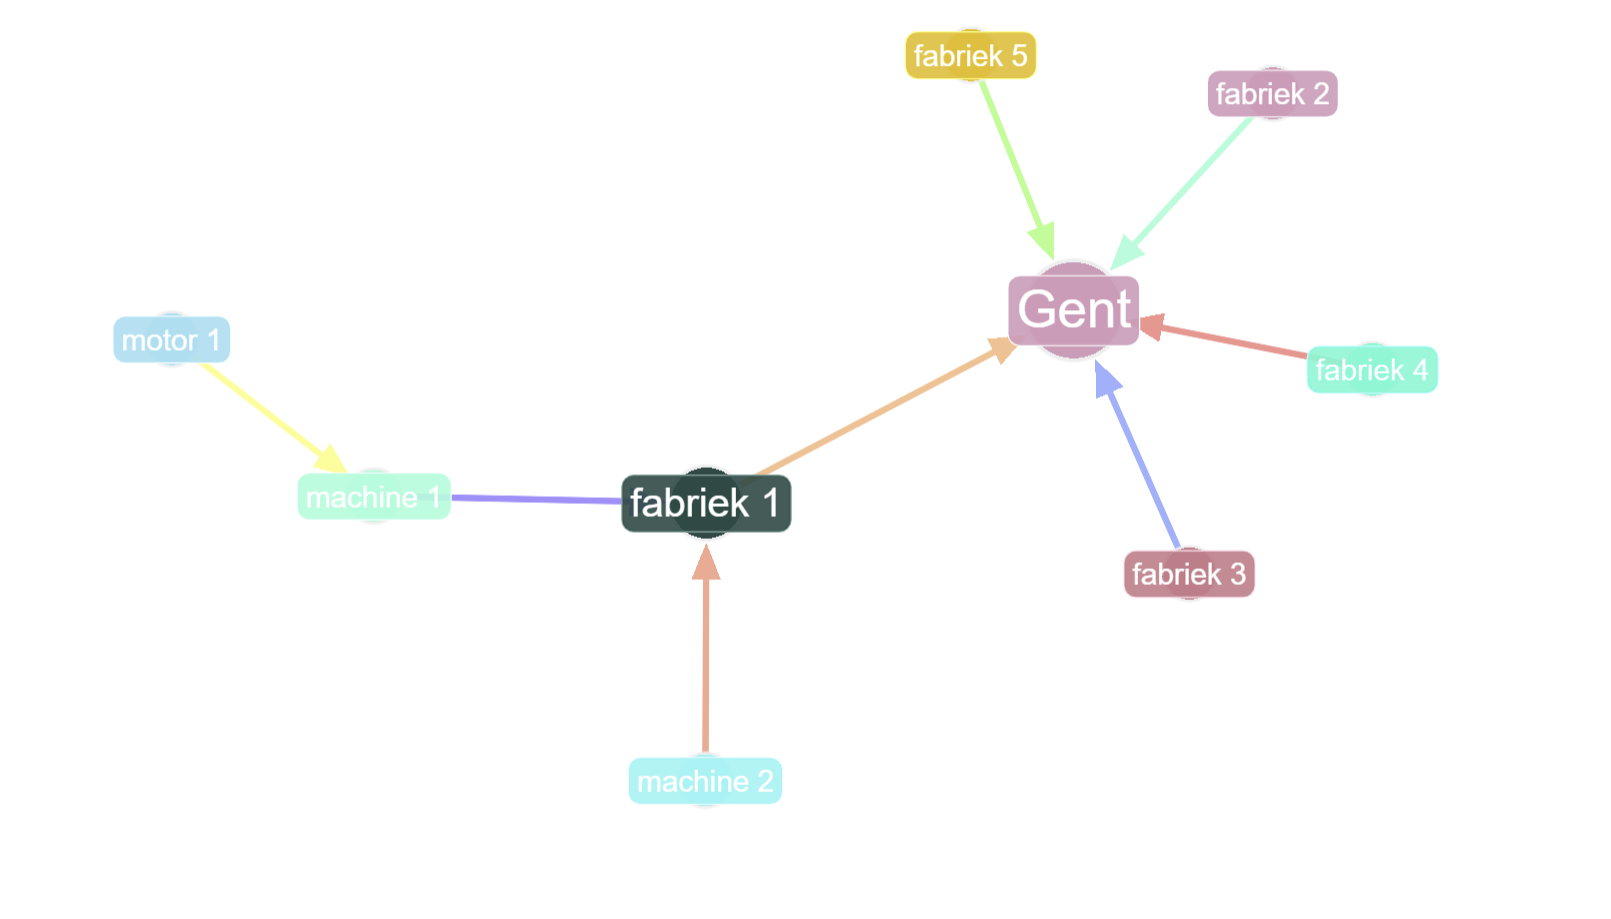
\includegraphics[width=0.8\textwidth]{./img/grapmodel_example.png}
     \caption[Voorbeeld Grafiekmodel.]{\label{fig:graphmodel}Voorbeeld van kleinschalig grafiekmodel, gemaakt met mock data.}
\end{figure}

\subsection{CosmosDB}
Cosmos DB is een NoSQL-database van het Microsoft Azure ecosysteem. Het biedt een lage latentie, is beschikbaar voor verschillende API's en kan grote hoeveelheden data verwerken met een hoge beschikbaarheid, wat belangrijk is in ons project~\autocite{CosmosDB2024}.
Daarnaast is CosmosDB horizontaal schaalbaar, wat betekent dat er op hoogtepunten tot een miljoen lees- en schrijfaanvragen kunnen verwerken door het benodigde aantal servers toe te voegen.
De hoge beschikbaarheid wordt gegarandeerd door replicatie, waardoor er snel kan worden overgeschakeld als er een probleem is in onze database.
Binnen ArcelorMittal wordt gebruik gemaakt van onder andere de Azure omgeving van Microsoft, waardoor CosmosDB een logische keuze is voor ons project.
CosmosDB ondersteunt verschillende API's zoals SQL, MongoDB, Cassandra, Gremlin en Table API, waardoor er flexibel kan worden gewerkt met verschillende soorten data.
In deze thesis wordt gebruik gemaakt van CosmosDB, omdat dit een grafiekdatabase bevat die ons in staat stelt om de data te structureren en te doorzoeken op basis van de relaties tussen de verschillende knopen.
Om op een later moment verbanden te kunnen leggen tussen processen binnen ArcelorMittal Gent, is dit onderdeel noodzakelijk voor het project.
Om de queries uit te voeren op CosmosDB wordt er gebruik gemaakt van de Gremlin API, deze API wordt uitgebreid besproken in~\ref{sec:gremlin}.
Voor deze thesis is er gebruik gemaakt van Azure database voor CosmosDB, die een gratis tier heeft met een beperkte hoeveelheid Request Units (RU's) per seconde.
In productie zou er gebruik gemaakt worden van de betaalde versie van CosmosDB, die meer Request Units (RU's) per seconde kan verwerken en meer opslagcapaciteit biedt.

\subsubsection{Request Units (RU)}
Cosmos DB werkt met Request Units (RU's), een abstracte maat voor de hoeveelheid systeembronnen (zoals CPU, geheugen en I/O) die nodig zijn om een bepaalde bewerking of query uit te voeren~\autocite{Brown2024}.
Elke bewerking krijgt een aantal Request Units toegewezen afhankelijk van de complexiteit en de gebruikte API, zegt~\textcite{Brown2024}.

Bij het bekijken van de monitoring van de Cosmos Database, werd er voor een query zoals ``Geef alle kranen met een alert op de motor'' ongeveer 10 RU's gerekend.
Voor dit onderzoek is er minder rekening gehouden met de RU's, aangezien er met een kleine dataset gewerkt wordt en de kosten veel lager zullen zijn dan in een productieomgeving.
Daarnaast maakt het aantal gebruikers ook een aanzienlijk verschil in de kosten, wat op dit moment nog niet kan worden ingeschat.

Bij Microsoft Azure zijn er verschillende manieren om te betalen voor verbruik (of RU’s) in Cosmos DB, afhankelijk van het benodigde schaalmodel:
\begin{itemize}
     \item Bij provisioned throughput reserveer je een vast aantal Request Units per seconde (RU/s), waarvoor je betaalt ongeacht of je ze volledig gebruikt. Dit model is geschikt voor toepassingen met een constante of voorspelbare belasting~\autocite{provisioned2024}.
     \item Bij serverless throughput betaal je enkel voor het aantal RU’s dat effectief verbruikt wordt. Aan het einde van de facturatieperiode wordt het totale verbruik aangerekend. Dit model is ideaal voor sporadisch gebruik of ontwikkelomgevingen met een lage belasting~\autocite{serverless2025}.
     \item Met autoscale throughput stel je een maximumcapaciteit in, waarna Cosmos DB automatisch schaalt tussen 10\% en 100\% van die waarde, afhankelijk van de werkelijke belasting~\autocite{autoscale2024}. Het voordeel van autoscale throughput is dat je geen handmatige schaling hoeft te doen. Een nadeel daarentegen is dat je altijd minimaal 10\% van de ingestelde maximumwaarde betaalt, wat bij lage activiteit duurder kan uitvallen dan het serverless model.
 \end{itemize}


\subsection{API:\@ Apache Gremlin}{\label{sec:gremlin}}
Om ervoor te zorgen dat de data kan opgehaald en bevraagd worden in CosmosDB wordt de Gremlin API van Apache TinkerPop gebruikt~\autocite{Tinkerpop2023}.
Apache TinkerPop is een framework voor grafiekberekeningen, dat gebruikt wordt voor grafiekdatabases en grafiekanalyses.
De API van Gremlin is gebasseerd op een REST API die communiceert tussen de database en de chatbot, waardoor er na bevraging een antwoord gegeven wordt met de gegevens uit deze database~\autocite{Medina2021}.
De taal bevat verschillende varianten voor verschillende programmeertalen zoals Gremlin-Java, Gremlin-Python en Gremlin-Groovy.
In ons geval zal Gremlin-Javascript gebruikt worden om de data in CosmosDB te bevragen, aangezien de databaseverbinding via Javascript geinitialiseerd wordt. 
Hiernaast is ook Neo4J overwogen met cypher als query taal, maar deze heeft zijn eigen ecosysteem en is niet even flexibel en schaalbaar als Gremlin API.\@
Gremlin daarentegen voorziet dat alle databases die TinkerPop-enabled zijn, kunnen worden gebruikt. Dit zijn databases die ondersteund worden door het Apache TinkerPop framework.
Hieronder vallen onder andere Amazon Neptune, CosmosDB, JanusGraph en nog vele andere \autocite{Tinkerpop2023a}.
Via de Gremlin API worden kunnen er verschillende vragen worden gesteld aan de database en wordt de benodigde data opgehaald. 
Zo kan er gevraagd worden welke knopen er zijn, hoeveel uitgaande relaties er zijn en gezocht worden naar specifieke labels.
Een belangrijke notitie is dat Gremlin case-sensitive is, wat betekent dat de juiste hoofdletters moeten gebruikt worden in de queries.
Dit kan mogelijk problemen geven bij het ophalen van de data. Hiervoor zijn alle values in de database omgezet naar kleine letters via een klein Python script, zodat er geen problemen ontstaan met het ophalen van de data.
Daarnaast zijn er bepaalde sleutelwaarden die in CosmosDB ook de juiste hoofdletters moet hebben (zoals label en name), hiervoor is er een kleine lijst meegegeven aan de chatbot die de juiste hoofdletters bevat.
Om dit te doen zal er met Python alle keys opgehaald worden uit de database en opgeslagen worden in een lijst, daarna maakt het Large Language Model een query en kijkt hij voor elk woord of deze in de lijst aanwezig is.
Indien de string in de lijst staat, wordt de hoofdlettergevoeligheid behouden, anders wordt de string omgezet naar kleine letters.

In codefragment~\ref{fig:gremlin} is een voorbeeld te zien van een Gremlin query die de knopen verbonden met machine 1 ophaalt.
Zoals te zien in dit codefragment, is er een query voor het opschonen en een query na het opschonen van de hoofdlettergevoeligheid. 
Daarin is te zien dat alles wat in kleine letters moet staan ook in kleine letters staat.
Hierbij wordt gebruik gemaakt van de \texttt{outE} functie die de uitgaande relaties ophaalt van de knoop, en de \texttt{inV} functie die de inkomende knopen ophaalt.

\begin{listing} [H]
     \begin{minted}{SQL}
          -- Query voor het opschonen
          g.V().HAS('label', 'MACHINE 1').OUTE('IS_ASSOCIATED').INV()

          -- Query na het opschonen
          g.V().has('label', 'machine 1').outE('is_associated').inV()
     \end{minted}
     \caption[Voorbeeld Gremlin query]{\label{fig:gremlin}Voorbeeld van een Gremlin query die de knopen ophaalt uit de database.}
\end{listing}

\subsection{REST API}{\label{sec:restapi}}
Om de communicatie tussen de chatbot en de database te vergemakkelijken wordt er gebruik gemaakt van een REST API ofwel Representational State Transfer Application Programming Interface.
Een REST API is een manier om flexibel en lichtgewicht te communiceren tussen verschillende applicaties via HTTP-verzoeken \autocite{RESTAPI2021}.
Het is voor het eerst ontworpen door Roy Fielding in 2000 en is sindsdien een populaire manier geworden om webservices te bouwen.
Een REST API maakt gebruik van de CRUD-operaties ofwel de GET, POST, PUT en DELETE om gegevens op te halen, toe te voegen, bij te werken of te verwijderen.
Daarnaast is een REST API ook stateless, wat betekent dat elke aanvraag onafhankelijk is van de andere aanvragen en er geen informatie wordt opgeslagen.
Voor deze use case maken wordt er gebruik gemaakt een POST request waarbij de vraag van een gebruiker wordt doorgegeven.
Als antwoord komt er een JSON-object terug met de resultaten van de query uit de database.
Indien er een knoop of relatie ``verwijderd'' moet worden, moet er een DELETE request uitgevoerd worden, ook dit is mogelijk via de REST API.\@
Als nuance is het belangrijk dat een knoop of relatie noot echt verwijderd wordt, maar deze enkel markeren als verwijderd.

Het voordeel van een REST API is dat het platformonafhankelijk is en dat het gemakkelijk te integreren is met andere systemen.
Dit doordat de requests aangeroepen worden via HTTP, ofwel Hypertext Transfer Protocol~\autocite{HTTP25}.
Om hier niet te diep op in te gaan, is het belangrijk om te weten dat HTTP een protocol is dat gebruikt wordt om gegevens te verzenden over het internet.
Simpelweg stuur je bijvoorbeeld een POST request met de vraag van de gebruiker naar de server, en krijg je een antwoord terug van de server.

\subsection{Runtime: NodeJS}
NodeJS is een open-source JavaScript runtime-omgeving die de mogelijkheid biedt om JavaScript-code uit te voeren op een server~\autocite{NodeJS2022}.
Via NodeJS kan er een lokale server opgezet worden die de communicatie tussen de chatbot en de database mogelijk maakt.
NodeJS werkt via een Single-Threaded, Non-Blocking I/O model wat betekent dat er geen nieuwe threads worden aangemaakt voor elke request.
Door middel van Callbacks en Promises werkt NodeJS asynchroon, wat betekent dat de code niet wacht op een antwoord van een request maar ondertussen andere requests kan verwerken.
Dit is nodig omdat de data in grote hoeveelheden aanwezig kan zijn en er zo niet eindeloos gewacht hoeft te worden op een antwoord van de database.
Met event loops worden de requests in een wachtrij geplaatst en worden ze verwerkt wanneer de server klaar is met een andere operatie.
Daardoor is NodeJS zeer performant en schaalbaar voor het verwerken van grote hoeveelheden data.

De technologie is in 2009 ontwikkeld en geïntroceerd door Ryan Dahl en is sindsdien zeer populair geworden in de webontwikkeling. 
NodeJS werd later door grote bedrijven zoals Netflix, eBay \& Uber gebruikt voor hun back-end systemen.
Zoals eerder vermeld is het geen framework maar een runtime-omgeving. 
Er zijn in een schone installatie geen specifieke modules of bibliotheken aanwezig, waardoor het een zeer lichte en flexibele omgeving is om mee te werken.
Daarnaast zijn er wel een aantal standaardmodules (core modules) aanwezig zoals HTTP, File system en Path, die de basisfunctionaliteit bieden voor het opzetten van een server en het werken met bestanden.
Deze modules zijn vaak nodig om folders en bestanden te beheren, dat is ook de reden waarom deze modules `standaardmodules' worden genoemd~\autocite{Kumar2023}.
Naast deze standaardmodules zijn er ook veel externe modules beschikbaar via npm (Node Package Manager), die gebruikt kunnen worden om de functionaliteit van NodeJS uit te breiden.
Zo is er onder andere een module beschikbaar voor het werken met CosmosDB voor bijvoorbeeld de connectie, genaamd @azure/cosmos~\autocite{cosmosNodeJS25}.

Een van de nadelen van NodeJS is dat het single-threaded is, wat betekent dat het niet geschikt is voor CPU-intensieve taken.
Dit komt omdat NodeJS gebruik maakt van een event loop die de requests in een wachtrij plaatst en ze verwerkt wanneer de server klaar is met een andere operatie.
Hierdoor kan het zijn dat een request die veel tijd nodig heeft om te verwerken de andere requests blokkeert.
Sinds 2018 is er een nieuwe feature geïntroduceerd in NodeJS genaamd Worker Threads, dit maakt het mogelijk om multi-threaded te werken.
Daardoor kunnen de CPU-intensieve taken in een aparte thread verwerkt worden en wordt de main thread vrij houden voor andere requests.

\subsection{LLM runtime: Ollama}
Om later in deze bachelorproef onze chatbot op te bouwen wordt er gebruik gemaakt van Ollama, een wrapper die het mogelijk maakt om verschillende large language models te draaien op een lokale server~\autocite{Manandhar2025}. 
Dit is een open-source bibliotheek die verschillende vooraf getrainde modellen bevat zoals de Llama modellen van meta, phi modellen van Microsoft en nog veel meer.
Naast het gebruik van modellen op hun eigen server, kan er ook gebruik gemaakt worden van sommige Hugging Face modellen die lokaal of in de Docker container kunnen worden opgezet~\autocite{HuggingFace2024}.

Door dit grote aanbod aan bestaande pretrained modellen, kan er snel vergeleken en getest worden door deze op te halen van Ollama zelf.
Dat is een groot voordeel omdat deze thesis de scope niet legt op het ontwikkelen van een large language model die natuurlijke taal kan verwerken en of Gremlin Queries kan maken.
Wel wordt er gezocht naar het beste bestaande model voor het maken van Gremlin queries en verwerken van natuurlijke taal, mits de nodige finetuning. 
Dit is geen eenvoudige klus, dit omdat er verschillende Gremlin versies bestaan die een andere query syntax hebben en er geen specifieke modellen beschikbaar zijn voor het genereren van Gremlin queries.
Met behulp van Retrieval Augmented Generation en Elasticsearch is dit probleem deels verholpen, In hoofdstuk~\ref{sec:chatbot} wordt hier dieper op ingegaan.

Tijdens de testfase zijn er verschillende modellen getest geweest, zoals Llama, CodeLlama \& Phi-4.
De Llama modellen Llama2 en Llama3 waren redelijk goed in het omzetten van gegevens uit de database naar natuurlijke taal, maar hadden moeite met het genereren van Gremlin queries.
Daarnaast is er ook gekeken naar CodeLlama, die met de benodigde finetuning, vaak betere Gremlin queries kan genereren, maar minder natuurlijke antwoorden geeft op basis van de gekregen informatie uit de database.
Over het algemeen blijft het een uitdaging om Gremlin queries te genereren met een large language model, omdat deze modellen niet specifiek getraind zijn op Gremlin syntax.
In~\ref{sec:LORA} wordt er een manier besproken die het mogelijk maakt om een model te finetunen op Gremlin syntax, maar dit is niet verder onderzocht in deze thesis door de beperkte resources.

Als laatste is ook Phi-4 getest, dit is een model dat ontwikkeld is door Microsoft, dit model is performanter, en dus sneller, dan de Llama modellen en kan goed omgaan met de gekregen gegevens.
In het volgende hoofdstuk wordt dieper ingegaan op de verschillende modellen, hun resultaten en waarom er gekozen is voor een combinatie van twee verschillende modellen.

\subsubsection{Llama2}
Llama 2 is een open-source large language model ontwikkeld door Meta AI~\autocite{llama2}. 
Het model is beschikbaar in verschillende versies, variërend van 7 tot 70 miljard parameters, afhankelijk van de gekozen grootte.
Llama 2 is ontworpen om te concurreren met andere geavanceerde modellen zoals GPT-3.5 en GPT-4.
De training van het model is gebaseerd op een combinatie van supervised finetuning en reinforcement learning met menselijke feedback (RLHF).
Echter blijven er altijd uitdagingen zoals hallucinaties en bias die net als andere LLM's kunnen blijven optreden.

\subsubsection{Llama3}
Llama 3 is de opvolger van Llama 2 en is een state-of-the-art large language model dat is ontwikkeld door Meta AI~\autocite{Meta2024}.
State-of-the-art wil zeggen dat het model de nieuwste technieken en algoritmen gebruikt om de prestaties te verbeteren.
Llama 3 heeft een aantal verbeteringen ten opzichte van zijn voorganger Llama 2, waaronder een grotere dataset en een verbeterde architectuur.
Het model is ook, net als zijn voorganger, beschikbaar in verschillende versies. Variërend van 7 tot 70 miljard parameters, afhankelijk van de gekozen grootte.
Llama 3 heeft ook iets verbeterde codeereigenschappen zoals het geven van Python of Javascript code, maar tijdens het testen bleek dat het nog steeds moeite had met het genereren van Gremlin queries.
Het model zou evengoed of beter kunnen presteren als Phi-4, maar als er gekeken wordt naar grafiek~\ref{fig:MMLU} zien we dat het model voor dezelfde kwaliteit van antwoorden 5 keer zo groot is als Phi-4.
Hierdoor is het model ook veel zwaarder, trager en dus minder interessant om te implementeren in ons project.


\subsubsection{Phi-4}{\label{sec:phi4}}
Phi-4 is ook een state-of-the-art large language model dat is ontwikkeld door Microsoft en heeft 14 miljard parameters~\autocite{Kamar2024}.
Het doel van Phi-4 is dat het een compact, maar krachtig en snel model is dat kan concurreren met andere grote modellen, zoals Llama3 zoals hiervoor besproken.
De testen met Phi-4 tegenover andere grote modellen toonden aan dat het model sneller en goed presteerd in vergelijking met andere modellen op vlak van natuurlijke taal.
In figuur~\ref{fig:MMLU} worden de scores van de MMLU benchmark weergegeven, dit is een benchmark die verschillende onderwerpen aanpakt zoals coderen, wiskunde en taal.
Hieruit kan worden afgeleidt dat Phi-4 een hoge score heeft, maar zeer gelijkaardig loopt met het zwaarste model van Llama 3.
Dit betekent dat Phi-4 in ons geval een goede keuze is omdat het een lichtgewicht model is en ook goed presteert in ons scenario, mits finetuning met de nodige context.
Aangezien snelheid vaak belangrijk is, wordt er gebruik gemaakt van de Phi-4 14 miljard parameters versie, die ook nog eens gekwantiseerd is.
De gekwantiseerde versie is een geoptimaliseerde variant die minder rekenkracht en geheugen vereist, in ruil voor een minimale, meestal verwaarloosbare daling in taalmodelnauwkeurigheid~\autocite{Qdrant25}.

Volgens \textcite{microsoft2024phi4} is dit model geschikt om te gebruiken voor een chatbot, doordat het model makkelijk te finetunen is en de uitvoer dus makkelijk aangepast kan worden waar nodig.
Hierdoor kan het model context geven over de data, terwijl het model ook nog eens goed blijft presteren op taalniveau.
In de paper van \textcite{microsoft2024phi4} staan verschillende voorbeelden van hoe het finetunen kan worden aangepakt aan de hand van context.
Daarbij wordt volgende context in een tekstbestand meegegeven: ``Je bent een expert in het beantwoorden van vragen over CosmosDB.\@ De belangrijkste informatie die je kan gebruiken staat in het items object van de JSON response''.
Door de meertaligheid van dit model, waarbij het op 40 verschillende talen is getrained, kan ook de context in het Nederlands gegeven worden.
De beste prestaties zullen overigens in het Engels zijn, maar de resultaten in het Nederlands zijn ook zeer goed.
Met zeer goed bedoel ik dat het antwoord grammaticaal correct is en de juiste samenvatting geeft van de data die in de database aanwezig is.
Daarnaast klinkt het ook formeel en professioneel, wat mooi meegnomen is voor de omgeving waar de chatbot zal draaien.
Daarom wordt dit model gebruikt om de gekregen data uit het JSON antwoord te analyseren en een natuurlijk antwoord terug te geven.

\begin{figure}[H]
     \centering
     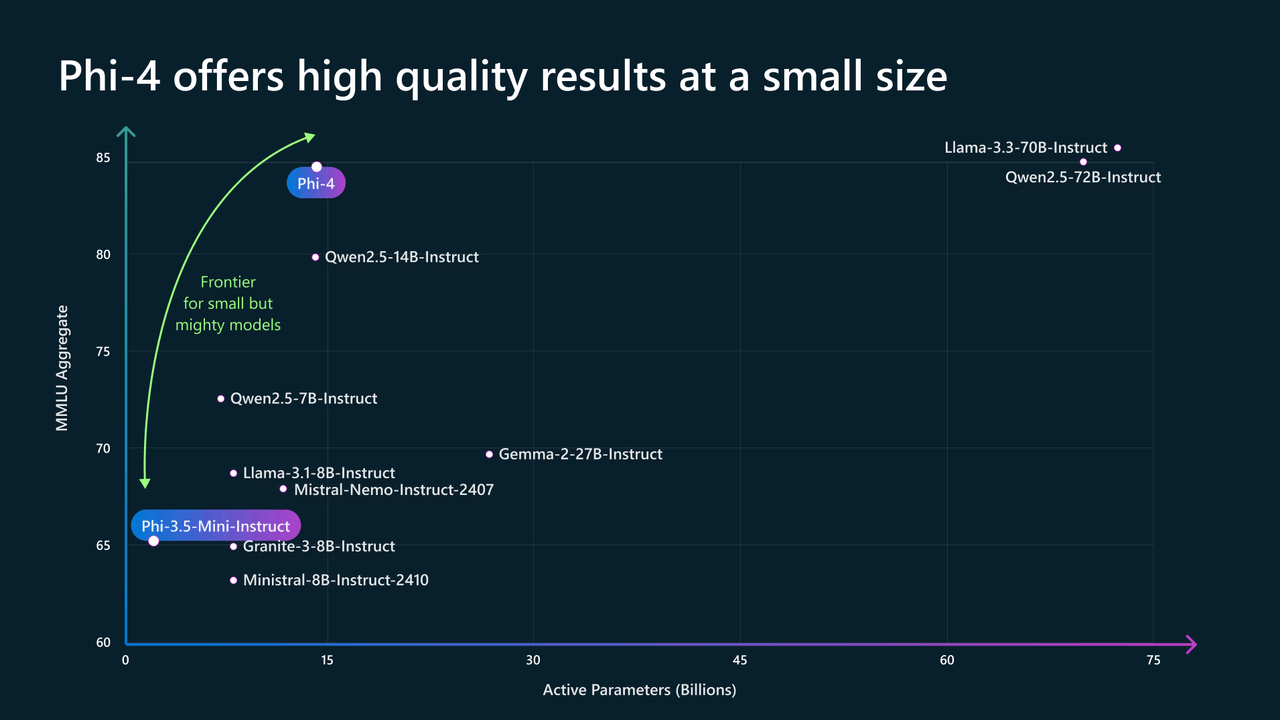
\includegraphics[width=0.8\textwidth]{./img/MMLU.png}
     \caption[benchmark LLMs.]{\label{fig:MMLU}Benchmark verschillende LLM's op de MMLU benchmark.}
\end{figure}

\subsubsection{CodeLlama}
Naast het Llama-model en Phi-4 is ook CodeLlama getest, dit is een open-source model dat is ontwikkeld door Meta AI en specifiek ontworpen is voor redenering en het genereren van code~\autocite{codellama}.
Het model is getraind op verschillende programmeertalen, zoals Python, JavaScript, C++ en vele andere. Voor het genereren van de Gremlin queries ligt het gebruik van dit model zeer voor de hand.
CodeLlama is in staat om beter te redeneren en functiekettingen te construeren, wat nodig is in Gremlin, mede dankzij de uitgebreide training op verschillende programmeertalen.\@
Door deze brede training kan het model de context van SQL-queries (zoals functies en variabelen) beter begrijpen en omzetten naar Gremlin queries.
Met functiekettingen wordt bedoeld dat de query opgebouwd is uit verschillende functies die elkaar opvolgen, zoals \texttt{V()} voor knopen op te halen \texttt{has()} waarbij specifieke sleutelwaarden gezocht kunnen worden.
Een voorbeeld hiervan is te zien in codefragment~\ref{fig:gremlin}.

Door voorbeeld-queries in een JSON bestand mee te geven aan het model, kan het de logica van SQL queries omzetten naar gelijkaardige Gremlin-structuren.
In deze thesis is er geopteerd om een JSON bestand te gebruiken aangezien dit een eenvoudige en snel begrijpbare manier is om de queries te structureren.
In de eerste testen is er gebruik gemaakt van een CSV bestand, maar deze bevatte vaak fouten, zoals verkeerde aanhalingstekens en komma's die de kolommen onnodig splitsten.
Bij een JSON bestand is dit probleem niet aanwezig, omdat de structuur duidelijk is en de data in een object wordt opgeslagen.
In de plaats van een kolom voor vraag en een kolom voor antwoord, bevat deze JSON een object met de vraag en het antwoord als sleutel-waarde paar.
Een voorbeeld hiervan staat in tabel~\ref{tab:RAGJSON}.

Voor de natuurlijke taal is dit model minder geschikt, het genereert vaak een technisch antwoord dat niet altijd even duidelijk is.
Het model bestaat in verschillende groottes, van 7B tot 70B parameters, afhankelijk van de use-case.
Daarnaast heeft het model ook verschillende versies zoals quantized en instruct versies~\autocite{HuggingFaceCodellama}.
De quantized versie is een versie die geoptimaliseerd is voor snelheid en geheugen, maar met een iets lagere nauwkeurigheid.
De instruct versie is een versie die geoptimaliseerd is voor opvolgen van instructies en codeer ondersteuning.
Wij maken gebruik van de 7B parameters-instruct versie die quantized is omdat deze instructies kan opvolgen, maar ook lichtgewicht is en voor weinig performantie problemen zal zorgen.
Dit model wordt ook alleen gebruikt voor het genereren van de Gremlin queries, daarna zal de gekregen data geanalyseerd worden door Phi-4 wat een sneller en lichter model is.

\begin{listing} [H]
     \begin{minted}{js}
          {
               "vraag": "Geef alle motoren",
               "antwoord": "g.V().has('name', containing('motor'))"
          },
     \end{minted}
     \caption[Voorbeeld van een JSON context bestand]{\label{fig:RAGJSON}Voorbeeld JSON met vraag en query.}
\end{listing} 

\subsection{Low Rank Adaptation (LoRA)}{\label{sec:LORA}}
Low Rank Adaptation (LoRA) is een techniek die het mogelijk maakt om grote taalmodellen te finetunen met een beperkte hoeveelheid data~\autocite{Cloudflare}.
In het begin van de thesis zijn er verschillende modellen besproken (zoals Phi-4 en CodeLlama) die gebruikt worden om natuurlijke taal te verwerken en vragen van een gebruiker om te zetten naar Gremlin queries.
Echter is Gremlin een zeer specifieke taal die niet altijd even makkelijk te genereren is door de verschillende versies van Gremlin.
LoRa maakt het mogelijk om doormiddel van een instructiedataset kleine stukjes toe te voegen aan een bestaand model om betere resultaten te krijgen.
Een machine learning model is namelijk een combinatie van algoritmen en een dataset.
Kort gezegd worden de bestaande matrices van het model bevroren en worden er extra matrices toegevoegd aaan bestaande gewichten doormiddel van low-rank matrixdecompositie, verteld~\textcite{Thiyagarajan2024}.
In figuur~\ref{fig:lora} is een voorbeeld te zien van hoe deze matrixdecompositie in zijn werk gaat.

Dit is een zeer interessante techniek die in de toekomst kan gebruikt worden om de resultaten van onze chatbot te verbeteren.
Deze techniek is in de huidige Proof of concept nog niet geïmplementeerd door een beperkte tijdsperiode voor de thesis en een te kort aan voldoende resources voor de training.

\begin{figure}[H]
     \centering
     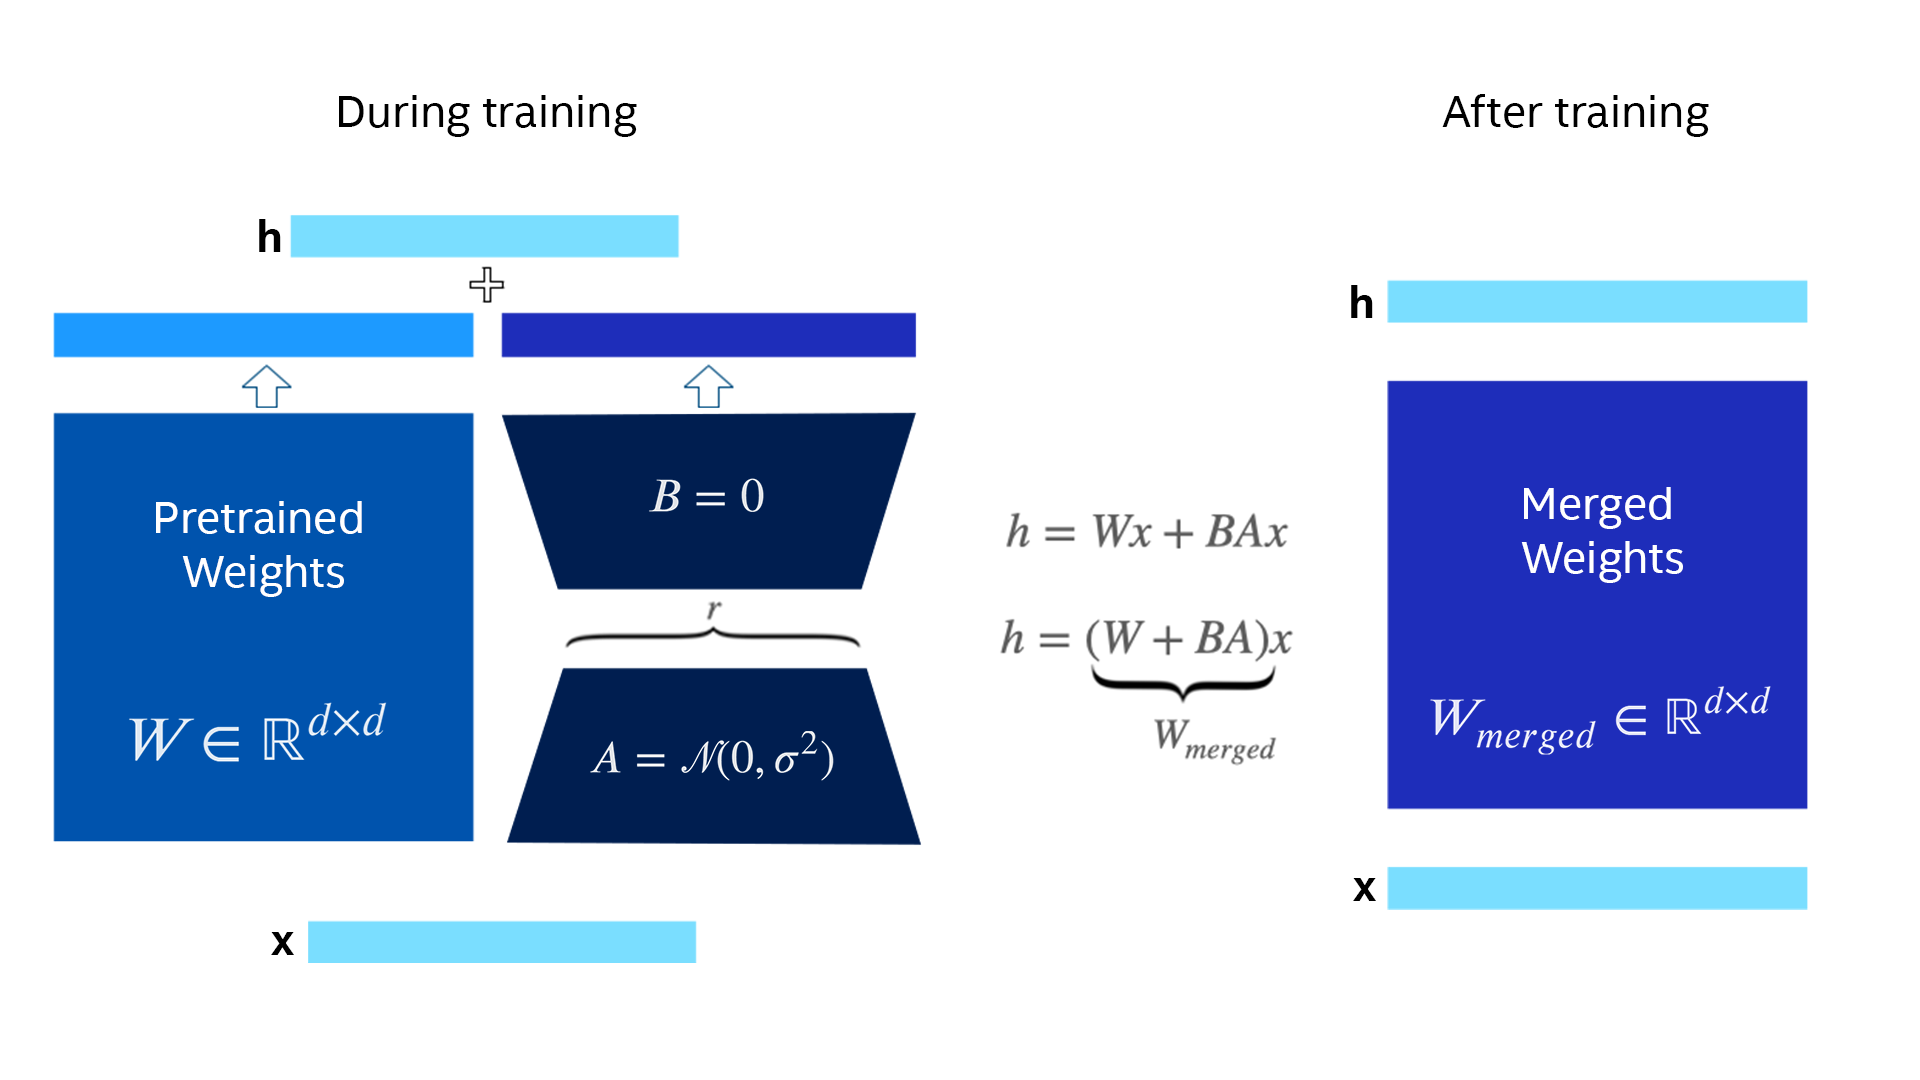
\includegraphics[width=0.8\textwidth]{./img/lora.png}
     \caption[Lora principe.]{\label{fig:lora}Afbeelding waar links pretrained model en rechts merged model is afgebeeld.}
\end{figure}

\section{Data preprocessing}
De data die gebruikt wordt komt uit een SAP-systeem. Deze data bevat een boomstructuur van de installatie op verschillende levels binnen ArcelorMittal Gent.
Dit houdt in dat de data in een hiërarchische structuur is opgebouwd, waarbij de verschillende processen met elkaar verbonden zijn.
Voor het ontcijferen van deze data zijn er verschillende specialisten binnen ArcelorMittal gecontacteerd die ons hebben geholpen met het vertalen van de sleutelwaarden in de JSON.\@
Alleen voor deze opsplitsing tussen locatie en machine is er een grote moeilijkheid. Doordat de dataset enorm groot is, en er soms handmatige aanpassingen gebeuren door werknemers, kan het zijn dat de levels van de hierarchie niet altijd correct zijn. 
Helaas kan er dus in dit onderzoek geen garantie gegeven worden door ArcelorMittal dat dit volledig klopt, na een handmatige controle lijkt dit naar schatting voor 90\% van de data te kloppen, maar als een afdeling uitgebreider is kan dit verschillen.
Dit betekent dat er voor verdere integratie een structurele aanpassing moet gebeuren aan de dataset en of de dataset moet opgeschoond worden.
Om de basis fundamenteel correct te houden, wordt er in de mock-data gewerkt met volgende hiërarchie:

\begin{itemize}
     \item level 1 in de boom, de locatie bijvoorbeeld Gent.
     \item level 2 de verschillende afdelingen zijn binnen Gent.
     \item level 3 de verschillende installaties zijn binnen de afdeling.
     \item level 4 de verschillende processen zijn binnen het proces.
     \item level 5 de verschillende machines zijn.
     \item > level 5 de verschillende onderdelen van de machines zijn.
\end{itemize}


\subsection{JSON}
De ontvangen data is in JSON-formaat, een veelgebruikte indeling voor het opslaan van gestructureerde gegevens.
JSON of JavaScript Object Notation is een tekstgebaseerde indeling die makkelijk te lezen en te schrijven is voor mensen en machines \autocite{Erickson2024}.
Doordat dit formaat zo flexibel is, is het een vaak gebruikte indeling bij web-, data- en software-applicaties.
Ondanks dat JavaScript in de naam van JSON zit is het een taal-onafhankelijk formaat dat ook in andere programmeertalen kan worden gebruikt.
Aangezien wij gebruik maken van JavaScript en Python is dit mooi meegenomen.

JSON werkt op basis van sleutel-waarde paren, waarbij de sleutel een unieke naam is die aan een waarde is gekoppeld.
De waarde kan eender welk type zijn zoals een string, nummer, boolean of zelfs een ander JSON-object waarin nog sleutel-waarde paren staan.
Hierdoor kan de data makkelijk gestructureerd en opgeslagen worden in een hiërarchische structuur.
De JSON data is al een zeer goed gestructureerd formaat, maar voor onze toepassing moeten deze data nog verder gestructureerd worden.
Dit houdt in dat de verschillende JSON-objecten gelinkt moeten worden aan elkaar, zodat de grafiek hieruit kan opgebouwd worden.
Daarvoor wordt JSON-LD gebruikt, een uitbreiding van JSON die het mogelijk maakt om data te structureren en te annoteren met semantische betekenis.

\subsection{JSON-LD}
JSON-LD staat voor JavaScript Object Notation for Linked Data. Dit is een uitbereiding van JSON die het mogelijk maakt om data te structureren en te annoteren~\autocite{jsonld.org}.
Het doel van deze Linked Data is om te zorgen dat je kan beginnen bij één object en van daaruit de embedded links kan volgen naar een andere object. 
Dit is vergelijkbaar met het grafiekmodel, waarbij er ook vanuit een knoop wordt vertrokken en er van daaruit verschillende relaties kunnen worden gevolgd.
In samenwerking met schema.org en GS1 (standaardnormen voor traceringsdata) kan deze data correct gestructureerd, genormeerd en gelinkt worden aan elkaar.
Het principe is hetzelfde, alleen wordt het model hier gecodeerd in code die makkelijk te lezen en te schrijven is voor mensen. 
Daarna kan deze JSON-LD direct worden ingelezen in CosmosDB om deze linken op te slaan en te visualiseren.
Deze linken zijn belangrijk aangezien er moet gevonden worden welke knopen aan elkaar verbonden zijn en welke dus invloed hebben op elkaar.

Er bestaan ook andere formaten zoals PYLD, dotNetRDF, \dots, maar doordat onze omgeving in JavaScript is opgebouwd en JSON-LD goed functioneert met Gremlin is dit een goede keuze.
Daarnaast zijn veel mensen bekend met JSON, waardoor implementatie en gebruik eenvoudiger zijn met enige technische kennis.

\subsection{JSON-LD tot Graph}
Om onze JSON-LD om te zetten naar een grafiekmodel wordt er gebruik gemaakt van JavaScript, waarbij de connectie wordt gemaakt met onze CosmosDB.\@
Door het gebruik van deze JavaScript-code, begint de conversie van de JSON-LD naar een grafiekmodel. Mits een goede vertaling van JSON naar JSON-LD, is dit een relatief eenvoudige taak.
Zo wordt er voor elke knoop een type toegevoegd, bijvoorbeeld als de knoop een fabriek is zal dit een \texttt{Place} zijn, als het een machine is zal dit een \texttt{Product} zijn.
Daarnaast is er ook de eigenschap label in de JSON-LD staan, dit wordt ook gebruikt om de knoop een naam te geven.
Hiervoor is er gekozen om het \texttt{ID} als \texttt{label} te gebruiken, dit is een unieke waarde die gebruikt wordt om de knoop te identificeren.
Naast het label worden ook andere eigenschappen toegevoegd aan de knoop die relevant zijn, zoals de alarmstatus van de knoop.\@

\section{Datemodellering en structuur}
\subsection{GS1}
GS1 is een wereldwijde organisatie die standaarden ontwikkelt voor identificatie, codering \& uitwisseling~\autocite{GS1standards}.
Dit zijn standaarden die bedrijven helpen om hun producten en diensten te identificeren, traceren en uit te wisselen.
Elk product heeft een unieke identificatiecode die het mogelijk maakt om het product te traceren doorheen de toeleveringsketen.
GS1 heeft verschillende standaarden ontwikkeld zoals de GTIN-code (Global Trade Item Number) en GLN-code (Global Location Number).
De GTIN-code is een code voor producten, waardoor elk product dat traceerbaar wil zijn een GTIN-code moet hebben. 
Indien de GTIN-code niet aanwezig is, kan het product niet worden geïdentificeerd en zal de fabrikant of leverancier dit moeten aanvragen bij GS1.
Ook locaties kunnen een unieke code krijgen, dit is de GLN-code. In volgende hoofdstukken wordt er dieper ingegaan op de ontwikkeling van de GTIN-code en de GLN-code, de rest van de GS1-standaarden zijn niet relevant voor dit onderzoek.
Momenteel zijn er geen GTIN-code's aanwezig in de mock-data, maar deze kan later worden toegevoegd aan de knopen die producten zijn.
Om deze codes te verkrijgen moet er een aanvraag gebeuren bij GS1, dit kan online via hun website.
Voor het maken van het grafiekmodel met de chatbot is dit momenteel minder relevant. 
Indien er wel GTIN of GLN codes aanwezig zijn in de data, kunnen deze toegevoegd worden als extra eigenschap of eventueel als label voor de knoop aangezien deze ook uniek zijn.

\subsubsection{GTIN}
De GTIN-code ofwel het Global Trade Item Number is een unieke identificatiecode die wordt gebruikt om producten te identificeren in de toeleveringsketen \autocite{GTIN2025}.
Deze bestaat uit 7 tot 11 cijfers benoemd met GTIN-8, GTIN-12, GTIN-13 en GTIN-14, de groote van de code hangt af van de toepassing en het type product.
Producten die klein zijn en weinig informatie bevatten kunnen een GTIN-8 hebben, terwijl grotere producten zoals dozen of pallets een GTIN-14 kunnen hebben.
In de gezondheidszorg wordt vaak een GTIN-14 ook toegelaten aangezien er ook veel informatie nodig kan zijn voor bijvoorbeeld medicatie.
De opbouw van de code is vrij simpel: de eerste 7 tot 11 cijfers identificeren het bedrijf, hoe korter deze prefix is, hoe meer producten er geïdentificeerd kunnen worden.
Na deze code volgt de productcode, dit is ook een reeks unieke cijfers voor identificatie van het product.
Als laatste volgt het controlecijfer, dit is een cijfer dat wordt berekend op basis van de andere cijfers in de code.
Dit cijfer wordt gebruikt om te controleren of de code correct is ingevoerd en of er geen fouten zijn gemaakt bij het scannen van de code.
Om een duidelijk voorbeeld te geven van deze GTIN-code, is er in figuur~\ref{fig:barcorde} een barcode te zien die een GTIN-12 code bevat.


\begin{figure}[H]
     \centering
     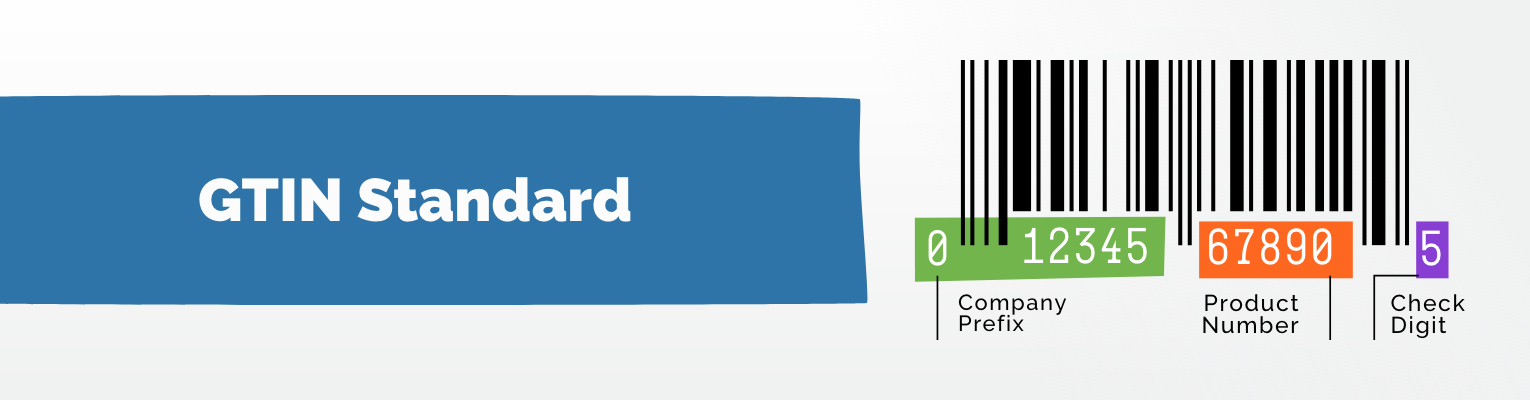
\includegraphics[width=0.8\textwidth]{./img/barcode_gtin12.jpg}
     \caption[GTIN-12 barcode]{\label{fig:barcorde} GTIN-12 barcode. }
\end{figure}

\subsubsection{GLN}
De GLN-code ofwel het Global Location Number is een unieke identificatiecode die wordt gebruikt om locaties te identificeren in de toeleveringsketen \autocite{GLN}.
Deze code is vergelijkbaar met de GTIN-code maar wordt gebruikt voor locaties, de opbouw is ook gelijkaardig.
De GLN code moet sinds 1 juli 2022 een uniek cijfer zijn en mag niet hergebruikt worden voor andere locaties.
Eerst is er de bedrijfsprefix, daarna volgt het adresnummer en als laatste een controlecijfer.
De bedrijfsprefix is een unieke code die wordt toegekend aan het bedrijf, deze code kan aanvraagd worden bij GS1. Het adresnummer is een unieke code die wordt toegekend aan de locatie, dit kan bijvoorbeeld een gebouw of een afdeling zijn.

\subsection{EPCIS-events}
Voor dit onderzoek wordt gebruik gemaakt van van EPCIS (Electronic Product Code Information Services), dit is een GS1-standaard die bedrijven in staat stelt om gebeurtenissen vast te leggen en te delen. 
Het biedt een gemeenschappelijk kader voor het vastleggen van de wat, wanneer, waar, waarom en hoe van gebeurtenissen die betrekking hebben op fysieke of digitale objecten. 
Deze waarden zijn ontwikkeld door GS1 om gegevens over beweging, status en verandering van een item in de toeleveringsketen (supply chain) vast te leggen en te delen binnen en buiten het bedrijf \autocite{Devins}.
``Met behulp van deze waarden kunnen we real-life objecten omzetten in elektronisch opgeslagen informatie, waarna we dit kunnen communiceren met eindgebruikers.`` zegt \textcite{Devins}.
Door deze normen toe te passen kan de traceerbaarheid van het product per proces gegarandeerd worden inclusief de gewenste parameters die opgeslagen worden in ons grafiekmodel zoals tijd (wanneer) en temperatuur (hoe), waar nodig.
Voor deze relaties goed en volgens de normen op te stellen, bestaan er EPCIS-events. Dit is een referentielijst waarin verschillende acties vooraf zijn bepaald.
Hierin staan bijvoorbeeld acties zoals ``add'', ``delete'' en ``update'' die gebruikt worden om de data te structureren en relaties aan te maken \autocite{Byun2020}.
Met de actie add wordt er een relatie toegevoegd met bijvoorbeeld het label IS\_ASSOCIATED en de tijdstempel van wanneer de associatie is aangemaakt.
Bijvoorbeeld als er een machine is met een bepaalde motor zullen de machine en de motor gekoppeld zijn met een EPCIS event IS\_ASSOCIATED die ook properties bevat zoals de tijdstempel van de associatie.
Bij deze actie worden ook properties toegevoegd in een event-lijst, daar wordt bepaald om welk soort event het gaat en worden eventuele extra parameters toegevoegd voor op de relatie, zoals de tijd van het event.
In codefragment~\ref{fig:jsonld} is een voorbeeld te zien van een associatie-event tussen een machine en een component.

De belangrijkste voordelen volgens \textcite{GS12025} staan opgelijst in tabel~\ref{tab:epcis-voordelen}.
\begin{table}[H]
    \centering
     \begin{tabular}{lp{0.6\textwidth}}
          \toprule
          \textbf{Voordeel} & \textbf{Beschrijving} \\
          \toprule
          Verbeterde zichtbaarheid & Door het vastleggen en delen van gedetailleerde gebeurtenisgegevens kunnen bedrijven beter inzicht krijgen in de bewegingen en status van producten in de toeleveringsketen. \\
          \midrule
          Efficiëntieverbeteringen & Door het automatiseren van gegevensverzameling en -uitwisseling kunnen bedrijven operationele efficiëntie verbeteren en fouten verminderen. \\
          \midrule
          Naleving van regelgeving & EPCIS helpt bedrijven te voldoen aan wettelijke vereisten voor traceerbaarheid en rapportage. \\
          \midrule
          Betere samenwerking & Door het delen van gebeurtenisgegevens met partners kunnen bedrijven beter samenwerken en de toeleveringsketen optimaliseren. \\
          \bottomrule
     \end{tabular}
     \caption[Belangrijkste voordelen van EPCIS volgens GS1]{\label{tab:epcis-voordelen}}
\end{table}


\subsection{Schema.org}
Schema.org is een grote verzameling van gestructureerde data die entiteiten (knopen) en relaties kan weergeven~\autocite{Douglas2023}.
GS1 en schema.org zijn complementair aan elkaar, aangezien GS1 zich richt op de identificatie en codering van producten en schema.org zich richt op de semantische betekenis van data.
In dit project worden objecttypen uit schema.org gecombineerd met concepten van GS1 om onze data gestructureerd en semantisch rijk te modelleren.
Met semantisch rijk wordt bedoeld dat de data meer betekenis krijgt, zo is er van schema.org \texttt{containedInPlace} eigenschap gebruikt om de relatie tussen een locatie en een asset te definiëren.
Van GS1 worden de EPCIS-events gebruikt om de acties te definiëren die uitvoerd worden op de data, zoals het toevoegen van een relatie of het verwijderen van een relatie.

Elke locatie krijgt een type, een label en extra properties zoals een adres of een geografische locatie.
Dit type of ID kan bijvoorbeeld \texttt{Place} zijn voor een locatie of \texttt{Product} voor een asset. 
Op de website van schema.org zijn alle mogelijkheden beschikbaar om de data te structureren en te annoteren.

In codefragment~\ref{fig:jsonld} is een voorbeeld te zien van een JSON-LD bestand met gegevens volgens schema.org in het eerste JSON-object.
Voor de locatie van Gent hebben is er ID 123, is het type een plaats en kan de vorige knoop teruggegeven worden met containedInPlace.
Verder kunnen properties toegevoegd worden zoals eronder aangegeven met een key-value paar.
% In het codeblok \ref{lst:jsonld} is een voorbeeld te zien van een JSON-LD bestand met gegevens.
\begin{listing}[H]
     \begin{minted}[fontsize=\footnotesize]{jsonld}
          {
          "@context": {
               "schema":"https://schema.org",
               "epcis": "https://ref.gs1.org/epcis/",
               "cbv": "https://ref.gs1.org/cbv/"
          }
               "@graph": [
                    {
                         "@id": "123",
                         "@type": "Place",
                         "name": "Gent",
                         "label": "Gent",
                         "schema:containedInPlace": 321,
                         "KEY": "VALUE"
                    },
                    {
                         "@type": "epcis:EPCISDocument",
                         "schemaVersion": "2,0",
                         "creationDate": "2025-03-19T17:40:54Z",
                         "epcis:EPCISBody": {
                              "epcis:EventList": {
                                   "epcis:AssociationEvent": {
                                   "eventTime": "2025-03-19T17:40:54Z",
                                   "eventTimeZoneOffset": "+01:00",
                                   "parentID": ["Machine 1"],
                                   "childEPCs": [
                                        [
                                        "Motor 1",
                                        "Motor 2"
                                        ],
                                   ],
                                   "action": "ADD",
                                   "disposition": "cbv:disp:active"
                                   }
                              }
                         }
                    }
               ]
          }
     \end{minted}
     \caption[Voorbeeld JSON-LD bestand]{\label{fig:jsonld}Voorbeeld van een JSON-LD bestand met locatiegegevens.}
\end{listing}


\section{Chatbot}{\label{sec:chatbot}}
De chatbot is een belangrijk onderdeel van ons project, aangezien het doorzoeken van de data zonder chatbot zeer tijdrovend en moeilijk is.
Dit zou eventueel kunnen gebeuren door zelf handmatig Gremlin queries te schrijven, maar dit is niet efficiënt en vereist veel technische kennis van de gebruiker.
De chatbot zal ons helpen om de data snel en efficiënt te doorzoeken en de juiste informatie te vinden.

In deze thesis is de chatbot een REST API die de vragen van de gebruiker kan beantwoorden op basis van de data die is verzameld.
Wat een REST API is en hoe deze werkt is al eerder besproken in sectie~\ref{sec:restapi}.
Om de vragen te beantwoorden worden twee verschillende modellen gecombineerd, namelijk Phi-4 en CodeLlama. 
Zoals eerder besproken in sectie~\ref{sec:phi4} is Phi-4 een large language model dat zeer goed is in het verwerken van natuurlijke taal en lichtgewicht is.
Daarnaast is er ook CodeLlama, dit model is specifiek ontworpen voor het genereren van code en kan goed omgaan met de Gremlin queries.
Om te zorgen dat de chatbot met beide modellen kan werken zijn er een aantal stappen ondernomen.

Eerst en vooral is de chatbot zelf in NodeJS opgezet, hierbij wordt er een runtime aangemaakt die bereikbaar is via bijvoorbeeld Postman.
Als volgt wordt er via deze JavaScript runtime een JSON object met de vraag aangemaakt zoals in codefragment~\ref{fig:userQuestion} te zien is.
Dit JSON object (de vraag) wordt dan teruggestuurd naar JavaScript, die op zijn beurt een Python script aanroept voor het genereren van een query.
Hier wordt gebruik gemaakt van Python omdat AI-modellen vaak beter ondersteund worden in Python en er veel bibliotheken beschikbaar zijn voor het werken met AI-modellen.
In dit Python-script wordt een functie aangeroepen die die context en voorbeeldqueries bevat, om zo'n beter en nauwkeuriger resultaat te ontvangen.
Hierdoor kan het model de Gremlin query genereren en deze teruggeven aan JavaScript.
Daarna wordt de Gremlin query uitgevoerd en wordt er een JSON object ontvangen met de resultaten.
Dit JSON object wordt dan doorgestuurd naar Phi-4 die de resultaten omzet naar natuurlijke taal en deze teruggeeft aan de NodeJS runtime.
Hierbij is het belangrijk dat de juiste context ook meegeven aan Phi-4, zodat hij de resultaten correct kan interpreteren.
Het JSON object bevat namelijk ook database informatie zoals de tijd van de query, wat niet relevant is voor de eindgebruiker en dus gefilterd wordt met deze extra context.

\begin{listing}[H]
     \begin{minted}{json}
          {
               "vraag": "Wat is de status van machine 1?",
          }
     \end{minted}
     \caption[Voorbeeld JSON vraag]{\label{fig:userQuestion}Voorbeeld van vraag in JSON.}
\end{listing}

\subsection{Retrieval Augmented Generation}
Om onze chatbot te optimaliseren wordt er gebruik gemaakt van RAG (Retrieval Augmented Generation).\@
Dit is een techniek die het mogelijk maakt om de chatbot te laten leren van de data die is verzameld in ongestructureerde teksten, databases of andere bronnen~\autocite{Zeichick2023}.
Hierdoor kan de chatbot beter begrijpen wat er van hem verwacht wordt en hoe hij de vragen moet beantwoorden zonder volledig het model te moeten hertrainen.
Dit is een low-level, maar veel gebruikte oplossing, die snel en flexibel bruikbaar is door documenten of context extra toe te voegen.

Hierbij wordt er een simpel tekstbestand met context aangemaakt waarbij de nodige informatie wordt meegegeven, zoals wat de functie is van het AI-model en wat belangrijk is of niet.
Daarnaast zijn er ook een aantal voorbeeldvragen en antwoorden toegevoegd via een JSON bestand, die geïndexeerd worden in een Elasticsearch cluster binnen de Docker container, dit principe wordt besproken in~\ref{sec:Elasticsearch}.
Dit is een belangrijke stap omdat de chatbot hierdoor beter kan begrijpen wat er van hem verwacht wordt en hoe hij de vragen moet beantwoorden.
Daarnaast is het belangrijk dat er in de context meegeven wordt dat hij geen tekst of codeblokken mag genereren maar enkel en alleen de query mag teruggeven.
Hiervoor is er ook een veiligheidsmechanisme gecodeerd dat ervoor zorgt dat query geen codeblok is zoals in markdown door de backtics te verwijderen.
Dit wordt gedaan door de query te filteren op backticks en alles voor en na deze backticks te verwijderen. Doordat LLM's vaak codeblokken genereren in markdown, is dit een belangrijke, maar eenvoudige stap.
Dit is belangrijke stap aangezien deze query direct moet geïmplementeerd worden in de database, wat betekent dat als er overige tekst of karakters in staan, dat het genereren zal mislukken door syntax fouten.
Indien een query succesvol uitgevoerd is, wordt deze query ook opgeslagen en in de JSON en toegevoegd aan de Elasticsearch-cluster.
Het is ook belangrijk dat hij de JSON resultset met items kan omzetten naar natuurlijke taal en begrijpt wat er wel of niet meegegeven mag worden.
Als voorbeeld is het zo dat er in het antwoord soms database performantiemetingen meegegeven worden die niet in het antwoord mogen staan voor de gebruiker.

Door al deze ``vereisten'' als context mee te geven aan de chatbot, kan hij beter begrijpen wat er van hem verwacht wordt en hoe hij de vragen moet beantwoorden.

\subsection{Elasticsearch}\label{sec:Elasticsearch}
Elasticsearch is een open-source, zoek en analyse-motor die gebruikt wordt voor het doorzoeken en analyseren van grote hoeveelheden data~\autocite{Elastic2025}.
Het is een gedistribueerde, RESTful zoekmachine die is gebouwd op Apache Lucene en een krachtige en flexibele manier biedt om gegevens te indexeren en doorzoeken.
Doordat Elasticsearch is gebouwd op een gedistribueerde architectuur, kan het grote hoeveelheden gegevens verwerken en snel resultaten teruggeven.
Met gedistribueerde architectuur wordt bedoeld dat de data en rekenkracht verdeeld kan worden over verschillende rekenbronnen, wat zorgt voor een betere schaalbaarheid en prestaties.
Elasticsearch wordt in deze thesis gebruikt om de JSON-data omtrent de Gremlin queries, op te slaan in een geïndexeerd cluster en snel te doorzoeken.
Elasticsearch indexeert en maakt tokens van de data, dit is een groot voordeel voor het stellen van de vraag aangezien er minder nauwkeurig gekeken wordt naar de volgorde van de woorden in de vraag, zegt \textcite{Oers2025}.
Door de Tokenisatie kan de chatbot ook vragen beantwoorden die niet letterlijk in de data staan, maar wel gerelateerd zijn aan de data.
Naast Tokenisatie, maakt Elasticsearch ook gebruik van een omgekeerde (of inverted) index, dit is een datastructuur die het mogelijk maakt om snel te zoeken naar documenten die bepaalde termen bevatten~\autocite{Brimley2023}.
In het volgende hoofdstuk wordt er dieper ingegaan op de Tokenisatie en de omgekeerde index die gebruikt worden in Elasticsearch.

Voor deze thesis wordt gebruik gemaakt van de Elasticsearch-package versie 8.12.0 in Python, deze versie is stabiel en ondersteunt de meeste functies die benodigd zijn.
De eerste testen met de laatste versie van Elasticsearch (9.0) gaven problemen met Python aangezien er op het moment van het schrijven nog geen Python client beschikbaar is voor deze versie.

\subsubsection{Tokenisatie}
Tokenisatie is een proces waarbij een tekst in kleine delen wordt gesplitst, deze delen komen terecht in een token stream die gebruikt wordt om te zoeken naar een bijpassend antwoord~\autocite{Elastic}.
Zo een tokenstream is de array met de verschillende woorden die in de vraag staan, dit wordt op zowel de vraag als de cluster toegepast.
De vraag is de vraag die de gebruiker stelt, de cluster is de verzameling van alle vragen die in de Elasticsearch-cluster staan.
Door deze token streams van vraag en cluster te vergelijken kunnen we met een threshold de relevantie bepalen om een juiste match te vinden.

\subsubsection{Omgekeerde index}
De omgekeerde index (of inverted index) is een lijst van alle tokens die in een vraag voorkomen, deze tokens krijgen in de omgekeerde index één of meer ID's toegewezen~\autocite{Vatsya2024}.
Deze ID's zijn unieke ID's die verwijzen naar de vraag die de token bevat. Hierdoor kunnen we enorm snel zoeken naar de juiste vraag en deze teruggeven aan de gebruiker.
De score van hoe relevant de vraag is wordt berekend op basis van TF (term frequency) en IDF (inverse document frequency).
Dit houdt in dat hoe vaker en hoe zeldzamer een token in een vraag is, hoe hoger de score zal zijn en dus hoe relevanter de vraag is.
In fragment~\ref{fig:invertedIndex} is een voorbeeld te zien van een zin omgezet naar omgekeerde index. 
Daar zal voor de vraag Toon alle machines in Gent gekozen worden voor de query die bij Geef alle machines in Gent hoort.
Dit omdat de frequency van de token ``machines en Gent'' in de vraag hoger is dan de andere tokens.

\begin{listing}[H]
     \begin{minted}{text}
          {
              Document 1: "Geef alle machines in Gent"
              Document 2: "Toon alle motoren in Antwerpen"

              tokens: ['Geef', 'alle', 'machines', 'in', 'Gent', 'Toon', 'motoren', 'Antwerpen']
               inverted index: {
                    'Geef': [1],
                    'alle': [1, 2],
                    'machines': [1],
                    'in': [1, 2],
                    'Gent': [1],
                    'Toon': [2],
                    'motoren': [2],
                    'Antwerpen': [2]
               }
          }
     \end{minted}
     \caption[Voorbeeld inverted index]{\label{fig:invertedIndex}Voorbeeld van een inverted index.}
\end{listing}

\subsection{Docker}
Docker is een open-source platform dat het mogelijk maakt om applicaties te ontwikkelen, en uit te voeren in containers~\autocite{docker2025}.
In deze thesis maken we gebruik van Docker om de verschillende componenten van onze chatbot te isoleren en te beheren.
Daarnaast zorgt het ervoor dat de omgeving van de applicatie consistent is, ongeacht waar deze wordt uitgevoerd.
Hierdoor kunnen we de applicatie eenvoudig implementeren en schalen zonder dat we ons veel zorgen hoeven te maken over de onderliggende infrastructuur.
Docker maakt gebruik van images die in containers worden uitgevoerd. Elke image kan meerdere containers hebben met hun eigen eigenschappen.
Docker is ook sneller en performanter dan traditionele virtuele machines omdat het geen volledige besturingssystemen hoeft te emuleren.
Met behulp van Docker kunnen we onze chatbot eenvoudig implementeren en laten communiceren met andere componenten zoals de Ollama modellen en Elasticsearch.

\subsubsection{Docker images}
Docker images zijn de basis van Docker containers, deze images bevatten alles wat nodig is om de applicatie uit te voeren~\autocite{Schmitt2024}.
Voor deze thesis hebben we een Dockerfile gemaakt die de basis image bevat en de benodigde dependencies installeert.
In figuur~\ref{fig:dockerfile} is een voorbeeld te zien van de Dockerfile voor NodeJS die we gebruiken om de chatbot te bouwen.

We maken in onze container

\begin{listing}[H]
     \begin{minted}{dockerfile}
          # Basis image
          # We gebruiken hier NodeJS versie 20
          FROM node:20

          # Bepalen van de werkdirectory (waar alle bestanden komen)
          WORKDIR /app

          # installeren van NodeJS packages
          COPY package*.json ./
          RUN npm install

          # Kopieer de requirements.txt naar de container
          # Dit is een tekstbestand met de Python packages die we nodig hebben
          COPY requirements.txt ./

          # Kopieer alle bestanden naar de container
          COPY . .

          # Commando om Python te installeren
          RUN apt-get update && apt-get install -y python3 python3-pip

          # Dependencies installeren die nodig zijn voor de chatbot
          RUN pip3 install --no-cache-dir -r requirements.txt

          # Starten van de Node.js applicatie
          CMD ["node", "scripts/chatbotPy.js"]
     \end{minted}
     \caption[Voorbeeld Dockerfile]{\label{fig:dockerfile}Voorbeeld van een Dockerfile.}
\end{listing}

\subsubsection{Docker containers}
Docker containers zijn geïsoleerde processen van een Docker image zonder dat het effect heeft op andere delen van het systeem, zegt~\textcite{Schmitt2024}.
Zo is er bijvoorbeeld een container voor de chatbot, een container voor Elasticsearch en een container voor de Ollama modellen, die simpel aan te roepen zijn via een API en kunnen communiceren met elkaar.\@

\subsubsection{Docker-compose}
Om alle containers in één keer op te starten en te beheren, maken we gebruik van Docker-compose~\autocite{docker2025}.
In figuur~\ref{fig:Docker-compose} is een voorbeeld te zien van een Docker-compose bestand dat gebruikt is om de verschillende containers op te starten.
Het gebruik van Docker-compose is vooral handig op kleine schaal, indien we de applicatie willen schalen naar een productieomgeving, kunnen we gebruik maken van Kubernetes.
Dit zorgt er namelijk voor dat de containers automatisch worden geschaald en kunnen worden beheerd.

\begin{listing}[H]
     \begin{minted}{yaml}
         version: '3.8'
          services:
          elasticsearch:
               image: docker.elastic.co/elasticsearch/elasticsearch:8.13.4
               container_name: elasticsearch
               environment:
                    - discovery.type=single-node
                    - ES_JAVA_OPTS=-Xms512m -Xmx512m
                    - xpack.security.enabled=false
                    - network.host=0.0.0.0
               
               
               volumes:
                    - es_data:/usr/share/elasticsearch/data

          chatbot:
               build:
                    context: ../..
                    dockerfile: scripts/docker/Dockerfile.chatbot
               container_name: chatbot
               command: ["node", "scripts/chatbotPy.js"]
               volumes:
                    - ../..:/app
               depends_on:
                    - elasticsearch
               ports:
                    - "3000:3000"

          ollama:
               container_name: ollama
               image: ollama/ollama:latest
               
               volumes:
               - ollama_models:/root/.ollama
               restart: unless-stopped
               environment:
               - OLLAMA_HOST=0.0.0.0

          volumes:
               es_data:
                    driver: local
               ollama_models:
     \end{minted}
     \caption[Voorbeeld Docker-compose]{\label{fig:Docker-compose}Voorbeeld van een Docker-compose bestand.}
\end{listing}